% !TeX spellcheck = en_US
\documentclass[fleqn]{article}

\usepackage[utf8]{inputenc}
\usepackage[slovak]{babel}
\usepackage[T1]{fontenc}
\usepackage{url}
\usepackage[hidelinks]{hyperref}
\usepackage{graphicx}
\usepackage{caption}
\usepackage{subcaption}
\usepackage{float}
\usepackage{amsmath}
\usepackage{xcolor}
\usepackage{array}
\usepackage{multirow}

\title{Biochemický reaktor - úvod}
\author{Matej Kintler}
\date{\today}

\begin{document}
	
\maketitle
\newpage

\tableofcontents
\newpage

\section{Uvod}

\newpage

\section{Biochemický reaktor}
\subsection{Základné informácie}
\input{content/ssec1}

\subsection{Typy bioreaktorov}
Na základe spôsobu prevádzky môže byť bioreaktor klasifikovaný ako vsádzkový, kontinuálny a polovsádzkový. 
Pri vsádzkovom spôsobe sa sterilné kultivačné médium naočkuje mikroorganizmami. Počas tohto reakčného obdobia sa s časom menia množstvá buniek, substrátu vrátane výživných solí, vitamínov a produktov. Fermentácia prebieha vopred stanovenú dobu a produkt sa zozbiera na konci.
V polovsádzkovom réžime sa do reaktora postupne pridávajú živiny, ako prebiehajú bioreakcie, aby sa získali lepšie výťažky a vyššia selektivita spolu s reguláciou reakčnej teploty. Produkty sa zbierajú na konci výrobného cyklu ako pri vsádzkovom bioreaktore. 
Charakteristickou črtou kontinuálneho bioreaktora je proces neustáleho dodávania substrátu. Prúd kvapaliny alebo suspenzie sa kontinuálne privádza a odstraňuje z reaktora. Na dosiahnutie rovnomerného zloženia a teploty je potrebné mechanické alebo hydraulické miešanie. Kultivačné médium, ktoré je buď sterilné alebo obsahuje mikroorganizmy, sa nepretržite dodáva do bioreaktora, aby sa udržal stabilný stav. Reakčné premenné a kontrolné parametre zostávajú konzistentné a vytvárajú v reaktore časovo konštantný stav. Výsledkom je nepretržitá produktivita.
Tradičné vsádzkové miešacie tankové reaktory (STR) a kontinuálne miešacie tankové
reaktory (CSTR) existujú už po stáročia a sú stále široko prijímané v chemickom a biologickom priemysle kvôli ich jednoduchosti. Ostatné bioreaktory, ktoré majú špeciálne konštrukčné a prevádzkové vlastnosti sú foto-bioreaktory, rotačné bubnové reaktory, hmlový bioreaktor, membránový bioreaktor, bioreaktory s náplňou a fluidnou vrstvou atď. Tieto boli navrhnuté tak, aby vyhovovali špecifickým procesom \cite{ref1}.


\subsection{Parametre opisujúce bioreaktor a ich význam}
Hlavné premenné, ktoré opisujú mikrobiálne procesy v prírode sú uvedené v Tabuľke \ref{tab: 1}.
%RP: Opat ``tab: 1'' nie je uplne najlepsi nazov. tag by mal informovat o obsahu, nie o umiestneny (ktore sa moze zmenit)

\textit{Množstvo mikroorganizmov} môže byť vyjadrené ako biomasa $(x)$ alebo počet buniek $(N)$ pri jednobunkových organizmoch (baktétrie, kvasinky, spóry) na jednotku pôdy, množstva vody, objemu alebo obsahu plochy. Vláknité organizmy (huby, aktinomycéty) sú charakterizované dĺžkou mycélia $(L)$ a počtom hýf $(n)$. Treba zdôrazniť, že $(n)$ nie je totožné s $(N)$, pretože vetvenie hýf skôr pripomína delenie buniek pri jednobunkových organizmoch. Vzťah medzi $(x)$, $(N)$ a $(L)$ nie je jednoznačný pretože hmota jednotlivých buniek a šírka hýf sa líši v závislosti od organizmu a podmieno rastu. Všeobecne možno povedať, že pri nadbytku výživných zlúčenín sa formujú veľké bunky resp. široké hýfy, zatiaľ čo pri hladovaní sa tvoria skôr menšie bunky alebo užšie hýfy. Výber biomasy $(x)$ alebo počet buniek $(N)$ alebo dĺžku mycélia $(L)$ závisí na danom prípade. Biomasa $(x)$ má očividnú výhodu pri skúmaní cyklu uhlíka a živín, zatiaľ čo počet buniek $(N)$ sa preferuje pri skúmaní populácie napr. výskyt mutácií alebo prenos plazmidov \cite{ref2}.

\begin{table}[H]
	\caption{Prehľad hlavných dynamických parametrov opisujúcich biochemický reaktor \cite{ref2}.}
	\label{tab: 1}
	\begin{tabular}{p{5cm} p{1.9cm} p{4cm}}
		\hline
		\textbf{Parameter} & \textbf{Symbol} & \textbf{Rozmer} \\ 
		\hline
		Hustota/koncentrácia biomasy & $x$ & $\mu g$ bunkovej hmoty na $g$ pôdy; $g$ bunkovej hmoty $m^{-2}$; $\mu g$ bunkovej hmoty na $mL$ vody\\
		Počet buniek & $N$ & $10^{6}$ buniek na $g$ pôdy; $10^{6}$ buniek na $mL$ vody\\
		Dĺžka mycélia & $L$ & $m$ na $g$ pôdy; $m$ na $mL$ vody\\
		Počet hýf & $n$ & $10^{6}$ na $g$ pôdy; $10^{6}$ na $mL$ vody\\
		Koncentrácia limitujúceho substrátu & $s$ & $mg$ na $g$ pôdy; $gm^{-2}$;$gL^{-1}$ vody\\
		Koncentrácia produktu & $p$ & $mg$ na $g$ pôdy; $gm^{-2}$;$gL^{-1}$ vody\\
		\hline	
	\end{tabular}
\end{table}

\textit{Koncentrácia limitujúceho substrátu} vo vode alebo v pôde, $(s)$, predstavuje množstvo esenciálnej živiny využívanej mikroorganizmami na rast a rozmnožovanie. Bežne nevieme posúdiť všetky potenciálne dostupné živiny a zameriať sa iba na jednu alebo zopár individuálnych zlúčenín alebo triedu molekúl, ktorá reprezentuje limitujúcu zlúčeninu, pretože chemoorganotrofné mikroorganizmy čerpajú energiu z organických zlúčenín, zatiaľ čo fotosyntetizujúce mikroorganizmy vyžadujú prísun svetla a zdroj fosforum dusíka a železa \cite{ref2}.

\textit{Množstvo produktov} $(p)$. Sem patria všetky medziprodukty a konečné produkty metabolizmu mikroorganizmov, ktoré vznikajú počas rastu. Typickými medziprodultmi sú organické kyseliny vznikajúce počas glykolýzy. Jediný konečný produkt aeróbnej mikrobiálnej dekompozície je oxid uhličitý, avšak pri anaeróbnych podmienkach vznikajú rôzne organické kyseliny, alkoholy, ketóny atď \cite{ref2}. 



\subsection{Matematické modely prietokového biochemického reaktora}
Najjednoduchším matematickým modelom, ktorý opisuje prietokový biochemický reaktor je tkz. Monod model. Tento model je veľmi obľúbený kvôli svojej jednoduchosti. Zakladá sa na dvoch predpokladoch: \text{1)} špecifická rýchlosť rastu buniek závisí od koncentrácie substrátu a  \text{2)} tvorba biomasy je spojená so spotrebou substrátu. Formulácia rovníc, ktoré popisujú materialovú bilanciu biomasy je nasledovná:
\begin{table}[H]
	\centering
	\begin{tabular}{ccccc}
		akumulácia & & množstvo & & množstvo \\
		bunkovej & = & vzniknutých & -- & odobraných \\
		hmoty & & buniek & & buniek \\
	\end{tabular}
\end{table}
\noindent a pre materialovú bilanciu substrátu platí:
\begin{table}[H]
	\centering
	\begin{tabular}{ccccccc}
		akumulácia & & množstvo & & množstvo & & množstvo\\
		substrátu & = & dodaného & -- & odobraného & -- & spotrebovaného .\\
		v systéme & & substrátu & & substrátu & & substrátu MO\\
	\end{tabular}
\end{table}
\noindent Ak uvažujeme, že objem reaktora sa nemení a prítok substrátu sa rovná odtoku suspenzie, potom môžme písať: 

\begin{equation} \label{eq:1}
	V\left(\frac{\,dx}{\,dt}\right) = V\mu(s)x - Fx,
\end{equation}
\begin{equation} \label{eq:2}
	V\left(\frac{\,ds}{\,dt}\right) = Fs_{in} - Fs - V\frac{1}{Y_{x}}\mu(s)x.
\end{equation}

\noindent Ak obe strany rovníc vydelíme objemom reaktora a označíme si pomer $\frac{F}{V} = D$, rýchlosť riedenia, môžme rovnice \ref{eq:1} a \ref{eq:2} upraviť do nasledovného tvaru:

\begin{equation} \label{eq:3}
	\frac{\,dx}{\,dt} = \left(\mu(s) - D\right)x, \text{kde}  \quad \mu(s) = \mu_{m}\frac{s}{K_{M} + s},
\end{equation}
\begin{equation} \label{eq:4}
	\frac{\,ds}{\,dt} = D\left(s_{in} - s\right) - \frac{1}{Y_{x}}\mu(s)x.
\end{equation}

\begin{table}[H]
	\centering
	\caption{Parametre Monod modelu, ich symbol a rozmer.}
	\label{tab: 2}
	\begin{tabular}{lll}
		\hline
		\textbf{Parameter} & \textbf{Symbol} & \textbf{Rozmer} \\
		\hline
		Špecifická rýchlosť rastu & $\mu(s)$ & $h^{-1}$ \\
		Maximálna špecifická rýchlosť rastu & $\mu_{m}$ & $h^{-1}$ \\
		Michaelisova konštanta & $K_{M}$ & $gL^{-1}$ \\
		Výťažok (biomasa) & $Y_{x}$ & \\
		Objem reaktora & $V$ & $L$ \\
		Prietok substrátu/suspenzie & $F$ & $Lh^{-1}$ \\
		Koncentrácia biomasy & $x$ & $gL^{-1}$ \\
		Koncentrácia substrátu & $s$ & $gL^{-1}$ \\
		Koncentrácia čerstvého substrátu & $s_{in}$ & $gL^{-1}$ \\
		\hline
	\end{tabular}
\end{table}

Rovnice \ref{eq:3} a \ref{eq:4} tvoria najjednoduchší opis biochemického reaktora -- Monod model, a význam jednotlivých parametrov je uvedený v Tabuľke \ref{tab: 2}. Avšak, tento model má množstvo nedostatkov. Nedokáže vysvetliť jednotlivé fázy rastu, ktoré sú pozorované experimentálne a to: lag-fázu, smrť buniek na základe hladovania, tvorbu produktu atď. Tieto nedostatky boli doplnené u tkzv. štruktorovaných modelov.

Model, ktorý berie do úvahy aj tvorbu produktu, získame doplnením Monod modelu do nasledovného tvaru: 

\begin{equation} \label{eq:5}
\frac{\,dx}{\,dt} = \left(\mu(s) - D\right)x,
\end{equation}
\begin{equation} \label{eq:6}
\frac{\,ds}{\,dt} = D\left(s_{in} - s\right) - \frac{1}{Y_{x}}\mu(s)x - \frac{1}{Y_{p}}\nu x,
\end{equation}
\begin{equation} \label{eq:7}
	\frac{\,dp}{\,dt} = \nu x - Dp,
\end{equation}

\noindent kde $p$ predstavuje koncentráciu produktu v $gL^{-1}$, $Y_{p}$ je bezrozmerný koefcient výťažnosti produktu a $\nu$ predstavuje kinetický člen rýchlosti tvorby produktu v jednotkách času napr. $ h^{-1} $. Do rovnice \ref{eq:4} sme doplnili časť, ktorá vraví, že časť substrátu sa spotrebuje na tvorbu produktu a rovnica \ref{eq:7} predstavuje obyčajnú materiálovú bilanciu produktu.

Ak by sme chceli do modelu zakomponovať tendenciu úmrtia mikroorganizmov počas hladovania, treba upraviť špecifickú rýchlosť rastu $\mu(s)$ tak, že bude obsahovať inhibičný člen $ K_i $, ktorého rozmer je $gL^{-1}$. Špecifická rýchlosť rastu potom nadobudne tvar:

\begin{equation} \label{eq:8}
	\mu(s) = \mu_{m}\frac{s}{K_{M} + s + \frac{s^2}{K_i}}.
\end{equation}


\section{Analýza matematických modelov}
V predchádzajúcej časti sme spomenuli viacero modelov, ktorými môžme opísať biochemický reaktor. V tejto časti sa budeme venovať analýze dvoch modelov a to Monod modelu doplnenému o produktovú časť a modelu, taktiež s produktovou časťou, ale s vplyvom inhibície.

\subsection{Dynamika}
Matematický model, ktorý opisuje bioreaktor je nelineárny model. To znamená, že odozva systému je rôzna pre rovnakú veľkosť skokovej zmeny. Túto nelinearitu si možno všimnúť na Obr. \ref{fig:1}. Ďalej si môžme všimnúť prudký narást koncentrácie produktu na počiatku, ktorý bol spôsobený nadbytkom biomasy a malým množstvom substrátu v systéme. Po ustálení dynamika produtku pripomímna systém 1. rádu. Na druhej strane v dynamike tvorby biomasy sa prejavuje nestabilná nula (menšie podkmity), ktoré sú spôsobené veľkou časovou konštantou tvorby biomasy a malou časovou konštantou odtoku suspenzie. V dynamike substrátu sa zasa prejavuje stabilná nula, ktorá opäť súvisí s rýchlym prítokom česrstvého média a pomalšou spotrebou na tvorbu biomasy a produktu.

\begin{figure}[H]
% RP: Ja vacsinou tieto identifikatory umiestnenia floatov ``[H]'' ani nepouzivam. Latex vie najlepsie ako umiestnovat obrazky/tabulky aby vysledny dokument vyzeral dobre
	\centering
	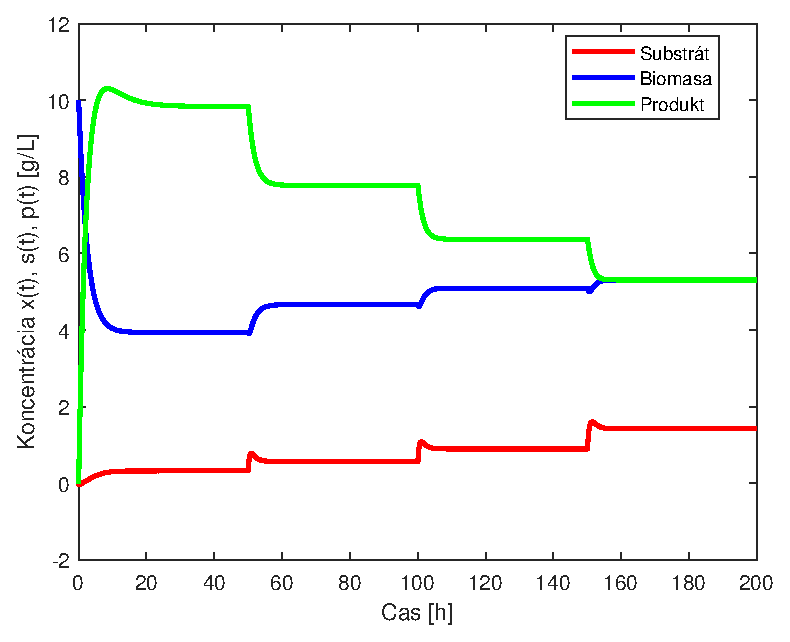
\includegraphics[width=1\linewidth]{images/step_change}
	% RP: Kvalita obrazku (aj dalsich) nie je nic moc. Zda sa mi, ze ma na okrajoch prilis vela bieleho miesta. Takisto je dost neostry. Neviem, aky sposob ukladania obrazkov z Matlabu pouzivate, ale skuste najst nejaky iny, resp. taky, ktory je vhodny pre pouzitie v Latexom generovanych dokumentoch. Internet urcite poradi. Ja to robi pomocou prikazu print, kde sa da stanovit priblizna velkost obrazku v samotnom dokumente a teda vysledok byva ostry. Hrubka ciar by mala byt aspon 2.
	\caption[]{Viacnásobná skoková zmena rýchlosti riedenia $D$ pri začiatočných podmienkach $p_0 = s_0 = 0, x_0 = 30 gL^{-1}$.}
	\label{fig:1}
\end{figure}

% Rp: ``Réžim'' -> ``Režim''
Réžim fungovania bioreaktora má významný vplyv na dynamiku celého systému a pri určitých podmienkach Monod model a model s inhibíciou môžu vykazovať rovnaké správanie, presne ako je tomu na Obr. \ref{fig:1}. Avšak, tieto modely sa odlišujú vo formulácii špecifickej rýchlosti rastu, ktorý má zásadný vplyv na dynamiku systému. Ako vidno na Obr. \ref{fig:2} pri Monod modely sa špecifická rýchlosť rastu limitne blíži ku maximálnej špecficikej rýchlosti rastu, zatiaľ čo model s inhibícou dosahuje svoje maximum v bode $S^{*} = \sqrt{K_M K_i}$. 

\begin{figure}[H]
	\centering
	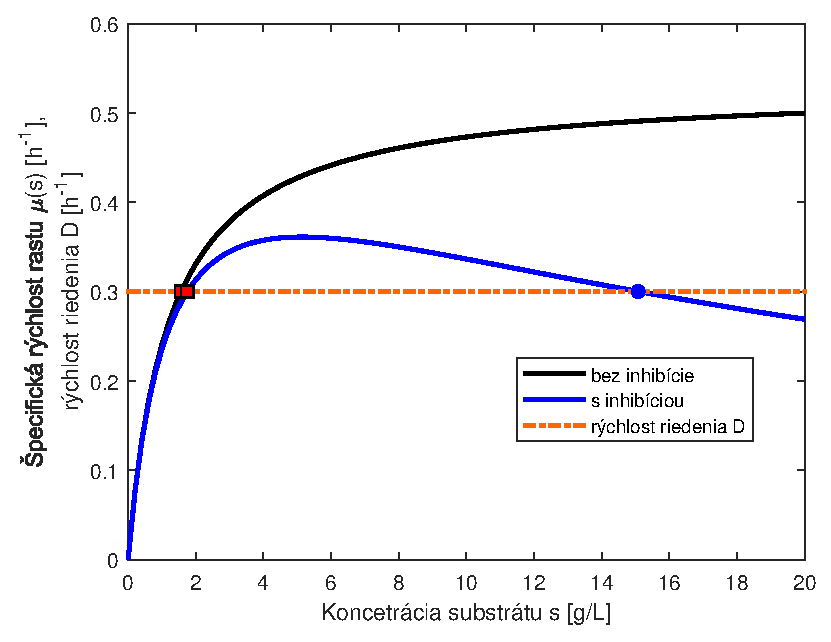
\includegraphics[width=1\linewidth]{images/spec_grow_rate_comparison}
	\caption[]{Porovnanie priebehu špecifickej rýchlosti rastu Monod modelu (červená) a modelu s inhibíciou (modrá). Červeným štvorčekom sú označené nenulové stabilné ustálené stavy, modrou guličkou je označený nestabilný stav.}
	\label{fig:2}
\end{figure}

\begin{figure}[H]
% RP: Tu uz na obrazkoch nie je vidiet skoro nic.
	\begin{subfigure}{.5\textwidth}
		\centering
		\includegraphics[width=1\linewidth]{images/dyn_wo_inhb}
		\caption[]{Monod model}
	\end{subfigure}
	\begin{subfigure}{.5\textwidth}
		\centering
		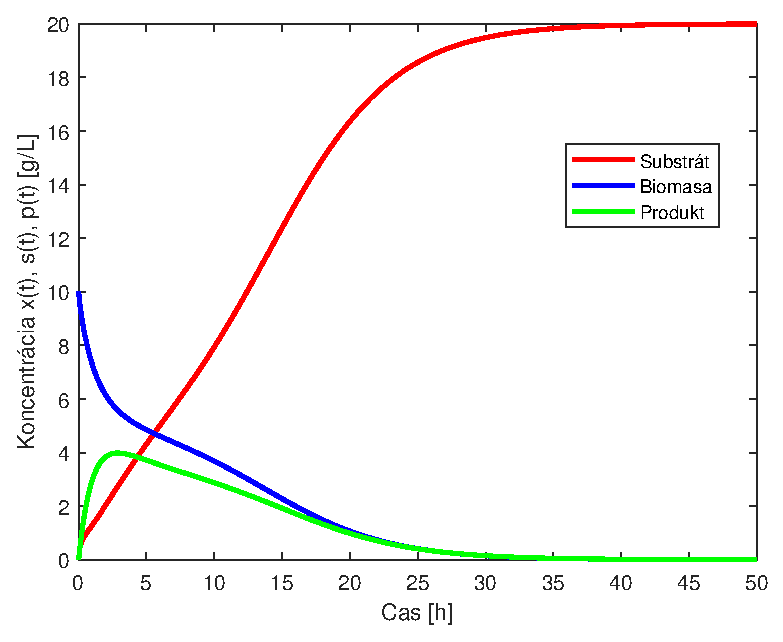
\includegraphics[width=1\linewidth]{images/dyn_inhb}
		\caption[]{Model s inhibíciou}
	\end{subfigure}
	\caption{Porovnanie dynamiky modelov pri rovnakých pracovných podmienkach.}
	\label{fig:3}
\end{figure}

\noindent Pri nesprávne zvolených pracovných podmienkach, či už počiatočných podmienkach systému, koncentrácie čerstvého substrátu alebo rýchlosti riedenia, model s inhibíciou bude vykazovať diametrálne odlišné správanie od Monod modelu, ako to je zobrazené na Obr. \ref{fig:3}.

\subsection{Stabilita}
Ustalene stavy pri roznych z.p. \\
Ustalene stavy pri roznych $s_{in}$ \\
Ustalene stavy pri roznych parametroch mu(s) a Ks \\

\section{Odhad parametrov}
\subsection{Optimalizacne metody}

\subsection{Pristupy k odhadu}
riesenie diff rovnic; pomocou diferencie

\section{Vysledky}

\section{Zaver}

\newpage
\bibliographystyle{plain}
\bibliography{literatura}

\end{document}